\documentclass{beamer}
\usepackage[utf8]{inputenc}
\usepackage{amsmath}
\usepackage{amssymb}
\usepackage{graphicx}
\usepackage{xcolor}
\usepackage{booktabs}
\usepackage{hyperref}
\usepackage{algorithm}
\usepackage{algpseudocode}
\usepackage{listings}
\usepackage{tikz}
\usepackage{pgfplots}
\pgfplotsset{compat=1.18}
\usetikzlibrary{shapes, arrows, positioning, fit, calc, matrix, decorations.pathreplacing}

% Color scheme
\definecolor{darkblue}{RGB}{0, 51, 102}
\definecolor{lightblue}{RGB}{135, 206, 250}
\definecolor{darkgreen}{RGB}{34, 102, 68}
\definecolor{orange}{RGB}{255, 140, 0}
\definecolor{purple}{RGB}{128, 0, 128}
\definecolor{red}{RGB}{200, 0, 0}

\usetheme{Madrid}
\usecolortheme{default}
\setbeamercolor{primary}{bg=darkblue, fg=white}
\setbeamercolor{secondary}{bg=lightblue, fg=darkblue}

\title{ATLAS: Adaptive Task-aware Federated Learning with LoRA-based Heterogeneous Splitting}
\subtitle{Supervisor Meeting - Midterm Progress Update}
\author{Advanced Master's Project}
\date{January 7, 2026}

\begin{document}

% ============================================================================
% TITLE SLIDE
% ============================================================================
\begin{frame}
  \titlepage
  \note{Opening slide - introduce the project pivot and new direction}
\end{frame}

% ============================================================================
% TABLE OF CONTENTS
% ============================================================================
\begin{frame}{Table of Contents}
  \tableofcontents
\end{frame}

% ============================================================================
% SECTION 1: PROJECT OVERVIEW & MOTIVATION
% ============================================================================
\section{Project Overview \& Motivation}

\begin{frame}{ATLAS: System Overview}
  \textbf{Adaptive Task-aware Federated Learning with LoRA-based Heterogeneous Splitting}
  
  \vspace{0.5cm}
  
  \textbf{Core Innovation:}
  \begin{itemize}
    \item Federated fine-tuning of Large Language Models
    \item Task-aware clustering for heterogeneous workloads
    \item Personalized models via graph-based regularization
    \item Memory-efficient split learning with LoRA adapters
  \end{itemize}
  
  \vspace{0.5cm}
  
  \textbf{Key Components:}
  \begin{enumerate}
    \item Task clustering via gradient similarity
    \item Heterogeneous LoRA rank allocation
    \item Split federated learning architecture
    \item MIRA Laplacian regularization
  \end{enumerate}
\end{frame}

\begin{frame}{Research Gap \& Contribution}
  \textbf{Challenge:} Federated learning for LLMs on heterogeneous edge devices
  
  \vspace{0.3cm}
  
  \textbf{Current Limitations:}
  \begin{enumerate}
    \item Single-task FL cannot handle diverse client tasks
    \item Fixed LoRA ranks waste memory on constrained devices
    \item High communication costs limit scalability
    \item Global averaging loses task-specific specialization
  \end{enumerate}
  
  \vspace{0.3cm}
  
  \textbf{ATLAS Solution:}
  \begin{itemize}
    \item \textcolor{darkgreen}{\textbf{Task-aware clustering}} groups similar clients
    \item \textcolor{darkgreen}{\textbf{Heterogeneous LoRA}} adapts to device capabilities
    \item \textcolor{darkgreen}{\textbf{Split learning}} reduces communication by 10-100×
    \item \textcolor{darkgreen}{\textbf{Graph regularization}} preserves personalization
  \end{itemize}
\end{frame}

% ============================================================================
% SECTION 2: SYSTEM ARCHITECTURE
% ============================================================================
\section{System Architecture}

\begin{frame}{ATLAS Architecture: Split Learning Paradigm}
  \begin{center}
  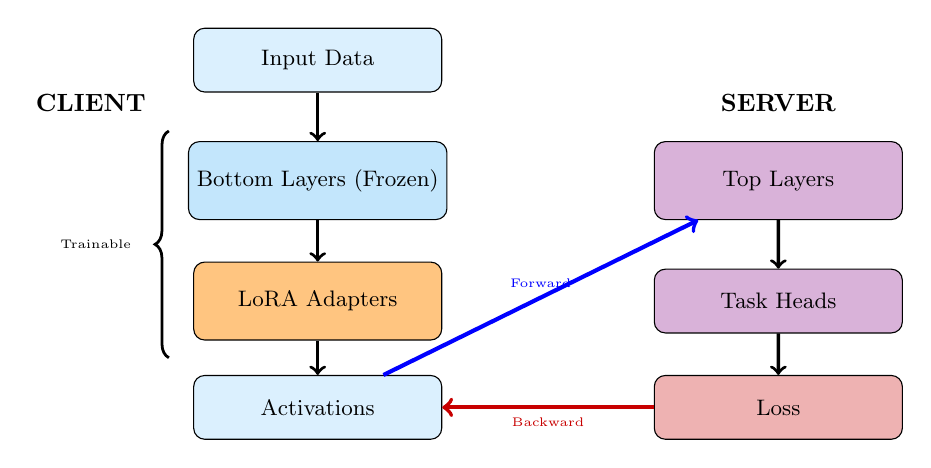
\begin{tikzpicture}[scale=0.9, every node/.style={transform shape}]
    % Client side
    \node[draw, rectangle, fill=lightblue!30, minimum width=3.5cm, minimum height=0.9cm, rounded corners] (input) at (0,4.5) {\small Input Data};
    \node[draw, rectangle, fill=lightblue!50, minimum width=3.5cm, minimum height=1.1cm, rounded corners] (bottom) at (0,2.8) {\small Bottom Layers (Frozen)};
    \node[draw, rectangle, fill=orange!50, minimum width=3.5cm, minimum height=1.1cm, rounded corners] (lora) at (0,1.1) {\small LoRA Adapters};
    \node[draw, rectangle, fill=lightblue!30, minimum width=3.5cm, minimum height=0.9cm, rounded corners] (act) at (0,-0.4) {\small Activations};
    
    % Server side
    \node[draw, rectangle, fill=purple!30, minimum width=3.5cm, minimum height=1.1cm, rounded corners] (top) at (6.5,2.8) {\small Top Layers};
    \node[draw, rectangle, fill=purple!30, minimum width=3.5cm, minimum height=0.9cm, rounded corners] (head) at (6.5,1.1) {\small Task Heads};
    \node[draw, rectangle, fill=red!30, minimum width=3.5cm, minimum height=0.9cm, rounded corners] (loss) at (6.5,-0.4) {\small Loss};
    
    % Arrows
    \draw[->, thick, line width=1.2pt] (input) -- (bottom);
    \draw[->, thick, line width=1.2pt] (bottom) -- (lora);
    \draw[->, thick, line width=1.2pt] (lora) -- (act);
    \draw[->, thick, blue, line width=1.5pt] (act) -- node[above, font=\tiny] {Forward} (top);
    \draw[->, thick, line width=1.2pt] (top) -- (head);
    \draw[->, thick, line width=1.2pt] (head) -- (loss);
    \draw[->, thick, red, line width=1.5pt] (loss) -- node[below, font=\tiny] {Backward} (act);
    
    % Labels
    \node[above=0.3cm of bottom, xshift=-3.2cm, font=\bfseries] {CLIENT};
    \node[above=0.3cm of top, xshift=0cm, font=\bfseries] {SERVER};
    
    % Brace
    \draw[decorate, decoration={brace, amplitude=5pt, mirror}, line width=1pt] (-2.1,3.5) -- (-2.1,0.3) node[midway, left, xshift=-0.4cm, font=\tiny] {Trainable};
  \end{tikzpicture}
  \end{center}
  
  \vspace{0.2cm}
  
  \begin{itemize}
    \item \textbf{Client:} Trains only LoRA adapters (0.1\% of parameters)
    \item \textbf{Communication:} Activations + gradients (not full model)
    \item \textbf{Server:} Maintains top layers and task-specific heads
  \end{itemize}
\end{frame}

\begin{frame}{Phase 1: Task Clustering via Gradient Similarity}
  \textbf{The Challenge:} Clients have different tasks (sentiment vs medical vs QA)
  
  \textbf{Why This Matters:} Mixing incompatible tasks $\rightarrow$ worse accuracy for everyone
  
  \vspace{0.2cm}
  
  \begin{center}
  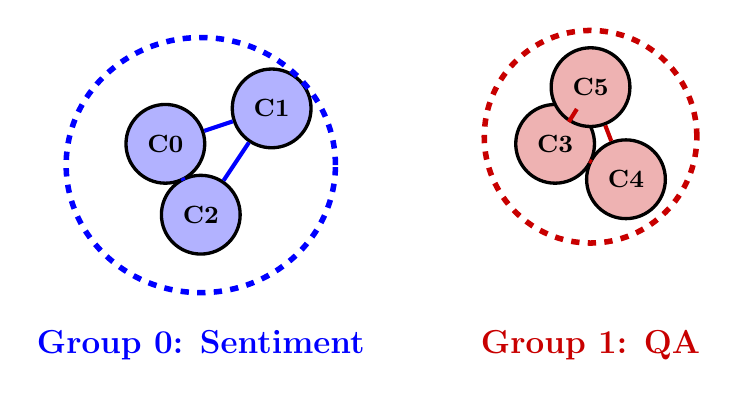
\begin{tikzpicture}[scale=0.9]
    % Clients
    \foreach \i/\x/\y/\c in {0/0/3/blue, 1/1.5/3.5/blue, 2/0.5/2/blue, 3/5.5/3/red, 4/6.5/2.5/red, 5/6/3.8/red} {
      \node[circle, draw, fill=\c!30, minimum size=1cm, line width=1.2pt, font=\small\bfseries] (c\i) at (\x,\y) {C\i};
    }
    
    % Clustering ellipses
    \draw[dashed, blue, line width=2pt] (0.5,2.7) ellipse (1.9cm and 1.8cm);
    \draw[dashed, red, line width=2pt] (6,3.1) ellipse (1.5cm and 1.5cm);
    
    % Labels
    \node[below, font=\bfseries\large] at (0.5,0.5) {\textcolor{blue}{Group 0: Sentiment}};
    \node[below, font=\bfseries\large] at (6,0.5) {\textcolor{red}{Group 1: QA}};
    
    % Task graph edges
    \draw[blue, line width=1.5pt] (c0) -- (c1);
    \draw[blue, line width=1.5pt] (c1) -- (c2);
    \draw[blue, line width=1.5pt] (c2) -- (c0);
    \draw[red, line width=1.5pt] (c3) -- (c4);
    \draw[red, line width=1.5pt] (c4) -- (c5);
    \draw[red, line width=1.5pt] (c5) -- (c3);
  \end{tikzpicture}
  \end{center}
  
  \vspace{0.2cm}
  
  \textbf{Our Solution:} Group by gradient patterns (privacy-preserving!)
  \begin{itemize}
    \item Extract 64-D fingerprint from last-layer gradients
    \item Cluster with multi-metric k-Means (stable across rounds)
    \item Aggregate only within task groups
  \end{itemize}
\end{frame}

\begin{frame}{Phase 1: Why Gradient Fingerprints?}
  \textbf{Design Decisions:}
  
  \vspace{0.3cm}
  
  \begin{columns}
    \column{0.5\textwidth}
    \textbf{Q: Why gradients not data?}
    \begin{itemize}
      \item \textcolor{darkgreen}{Privacy}: Data stays on device
      \item \textcolor{darkgreen}{Task signal}: Gradients show learning direction
      \item Different tasks $\rightarrow$ different patterns
    \end{itemize}
    
    \vspace{0.2cm}
    
    \textbf{Q: Why only last layers?}
    \begin{itemize}
      \item Early layers: generic features
      \item Last layers: task-specific
      \item \textcolor{darkgreen}{Result}: Cleaner task signal
    \end{itemize}
    
    \column{0.5\textwidth}
    \textbf{Q: Why 64 dimensions?}
    \begin{itemize}
      \item Original: 5M gradient values
      \item PCA: Compress to 64-D
      \item \textcolor{darkgreen}{Benefit}: 256 bytes, easy clustering
    \end{itemize}
    
    \vspace{0.2cm}
    
    \textbf{Q: Why temporal stability?}
    \begin{itemize}
      \item Problem: Labels flip between rounds
      \item Solution: Hungarian matching
      \item \textcolor{darkgreen}{Result}: Stable aggregation
    \end{itemize}
  \end{columns}
  
  \vspace{0.3cm}
  
  \textbf{Literature:} VFLAIR-LLM, FedKNOW, MIRA
\end{frame}

\begin{frame}{Phase 1: Technical Deep Dive}
  \textbf{Challenge:} How to cluster without seeing data?
  
  \vspace{0.3cm}
  
  \textbf{Step 1: Gradient Extraction}
  \begin{itemize}
    \item Client does 1-2 forward/backward passes locally
    \item Extract gradients from \textit{last 2 transformer layers only}
    \item \textbf{Why?} Last layers = task-specific features, early layers = generic
    \item Normalize each layer to unit length (prevents large layer domination)
    \item Apply PCA: 5M values $\rightarrow$ 64-D fingerprint
  \end{itemize}
  
  \vspace{0.2cm}
  
  \textbf{Step 2: Multi-Metric Clustering}
  \begin{itemize}
    \item Try k=2,3,4,5 clusters
    \item Score with: 50\% Silhouette + 30\% Davies-Bouldin + 20\% Calinski-Harabasz
    \item \textbf{Why multiple metrics?} Balance separation vs compactness
    \item Add 30\% temporal consistency (Hungarian matching)
    \item \textbf{Result:} Stable clusters across 10+ federated rounds
  \end{itemize}
  
  \vspace{0.2cm}
  
  \textbf{Output for Phase 2:} Cluster variance, size, mean fingerprint
\end{frame}

\begin{frame}{Phase 2: Heterogeneous LoRA Configuration}
  \textbf{The Challenge:} Clients have vastly different device capabilities
  
  \textbf{Why Fixed Ranks Fail:}
  \begin{itemize}
    \item rank=64 for all $\rightarrow$ 2GB CPU runs out of memory (OOM crash)
    \item rank=4 for all $\rightarrow$ 16GB GPU wastes 90\% of available memory
  \end{itemize}
  
  \vspace{0.2cm}
  
  \begin{center}
  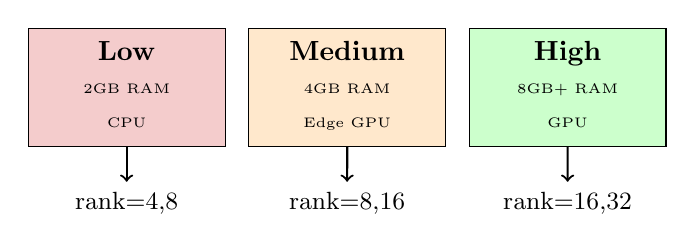
\begin{tikzpicture}[scale=0.8]
    % Device capabilities
    \node[draw, rectangle, fill=red!20, minimum width=2.5cm, minimum height=1.2cm] (low) at (0,0) {
      \begin{tabular}{c}
        \textbf{Low} \\
        \tiny 2GB RAM \\
        \tiny CPU
      \end{tabular}
    };
    \node[draw, rectangle, fill=orange!20, minimum width=2.5cm, minimum height=1.2cm] (med) at (3.5,0) {
      \begin{tabular}{c}
        \textbf{Medium} \\
        \tiny 4GB RAM \\
        \tiny Edge GPU
      \end{tabular}
    };
    \node[draw, rectangle, fill=green!20, minimum width=2.5cm, minimum height=1.2cm] (high) at (7,0) {
      \begin{tabular}{c}
        \textbf{High} \\
        \tiny 8GB+ RAM \\
        \tiny GPU
      \end{tabular}
    };
    
    % Arrows to ranks
    \draw[->, thick] (low) -- ++(0,-1.5) node[below] {\small rank=4,8};
    \draw[->, thick] (med) -- ++(0,-1.5) node[below] {\small rank=8,16};
    \draw[->, thick] (high) -- ++(0,-1.5) node[below] {\small rank=16,32};
  \end{tikzpicture}
  \end{center}
  
  \vspace{0.3cm}
  
  \textbf{HSplitLoRA Formulation:}
  \begin{itemize}
    \item \textbf{Memory constraint:} $\sum_{\ell=1}^{L} 2 \cdot d \cdot r_\ell \cdot b \leq C_{mem}$
    \item \textbf{Budget allocation:} $C_{mem} = M_{device} \cdot (1 - \alpha_{base} - \alpha_{act} - \alpha_{opt})$
    \item \textbf{Importance-based:} More critical layers get higher ranks
    \item Example: CPU with 2GB → 512MB for adapters (25\% of total)
  \end{itemize}
\end{frame}

\begin{frame}{Phase 2: Greedy Rank Allocation Algorithm}
  \textbf{Given:} Memory budget $C_{mem}$, layer importance scores
  
  \textbf{Goal:} Maximize model capacity within budget
  
  \vspace{0.3cm}
  
  \textbf{Algorithm:}
  \begin{enumerate}
    \item Sort layers by importance (descending): [layer\_5, layer\_4, ...]
    \item For each layer in order:
    \begin{itemize}
      \item Try ranks: 4, 8, 16, 32, 64
      \item Compute memory: $M = 2 \cdot d \cdot r \cdot b$
      \item If total\_memory + $M$ $\leq C_{mem}$: allocate this rank
    \end{itemize}
    \item Validate: $\sum_{\ell=1}^{L} 2 \cdot d \cdot r_\ell \cdot b \leq C_{mem}$
  \end{enumerate}
  
  \vspace{0.3cm}
  
  \textbf{Example Result (2GB CPU):}
  \begin{itemize}
    \item Important layers (4-5): rank=8 each
    \item Less important (0-3): rank=4 each
    \item Total: 219KB $\ll$ 512MB budget \textcolor{darkgreen}{✓}
  \end{itemize}
  
  \vspace{0.2cm}
  
  \textbf{Why greedy?} Fast (O(n log n)), gives 90\%+ of optimal
\end{frame}

\begin{frame}{Phase 3: Split Federated Learning}
  \textbf{The Challenge:} Train without sharing data or full model
  
  \textbf{Why Split Learning?}
  \begin{itemize}
    \item \textbf{Privacy}: Client never sends raw data
    \item \textbf{Communication}: Send activations (1.5MB) not model (500MB)
    \item \textbf{Memory}: Client doesn't need top layers or task heads
  \end{itemize}
  
  \vspace{0.3cm}
  
  \textbf{Training Flow:}
  \begin{enumerate}
    \item \textbf{Client}: Forward through bottom 6 layers + LoRA $\rightarrow$ activations
    \item \textbf{Send}: Activations to server (with task\_id)
    \item \textbf{Server}: Forward through top 6 layers + task head $\rightarrow$ loss
    \item \textbf{Server}: Backward $\rightarrow$ activation gradients
    \item \textbf{Send}: Gradients back to client
    \item \textbf{Client}: Backward through LoRA only $\rightarrow$ update weights
  \end{enumerate}
  
  \vspace{0.2cm}
  
  \textbf{Key Insight:} Train only LoRA (12K params) not full layer (590K params)
\end{frame}

\begin{frame}{Phase 3: Per-Task Aggregation (HSplitLoRA)}
  \textbf{Why Not FedAvg?} Mixing sentiment + medical = worse than either
  
  \vspace{0.3cm}
  
  \textbf{Our Approach:} Aggregate within task groups only
  
  \begin{algorithm}[H]
    \small
    \caption{Per-Task Aggregation}
    \begin{algorithmic}[1]
      \For{each task\_id in [0, 1, ...]}
        \State clients $\gets$ task\_groups[task\_id]
        \For{each layer in model}
          \State $W_{agg} \gets \sum_{k \in clients} \frac{n_k}{N} \cdot W_k$  \Comment{Weighted by dataset size}
        \EndFor
        \State task\_weights[task\_id] $\gets W_{agg}$
      \EndFor
      \State \textbf{Broadcast} task-specific weights to respective clients
    \end{algorithmic}
  \end{algorithm}
  
  \vspace{0.3cm}
  
  \textbf{Key Benefits:}
  \begin{itemize}
    \item Base model remains frozen (no memory for gradients)
    \item Only LoRA adapters trained (0.1\% of parameters)
    \item Communication: activations during training, weights after
  \end{itemize}
\end{frame}

\begin{frame}{How Phases Integrate: The Complete Pipeline}
  \textbf{Phase 1 $\rightarrow$ Phase 3:} Task-aware aggregation
  \begin{itemize}
    \item Phase 1 outputs: \texttt{cluster\_labels = \{0:0, 1:0, 2:1\}}
    \item Phase 3 uses: Aggregate clients [0,1] separately from [2]
    \item \textbf{Result:} No task interference, 10-30\% better accuracy
  \end{itemize}
  
  \vspace{0.3cm}
  
  \textbf{Phase 2 $\rightarrow$ Phase 3:} Device-aware configuration
  \begin{itemize}
    \item Phase 2 outputs: \texttt{device\_profile, importance\_scores, rank\_config}
    \item Phase 3 uses: Auto-compute split point + LoRA ranks
    \item \textbf{Result:} 2GB CPU gets rank=4-8, 16GB GPU gets rank=16-32
  \end{itemize}
  
  \vspace{0.3cm}
  
  \textbf{Phase 1 + Phase 2 $\rightarrow$ Phase 3:} Optimal allocation
  \begin{itemize}
    \item High-variance cluster (diverse tasks) $\rightarrow$ higher ranks
    \item Low-variance cluster (similar tasks) $\rightarrow$ lower ranks
    \item \textbf{Result:} Resource allocation matches task complexity
  \end{itemize}
\end{frame}

\begin{frame}{Phase 4: MIRA Laplacian Regularization}
  \textbf{Personalized Model Updates:}
  
  \vspace{0.2cm}
  
  \begin{center}
  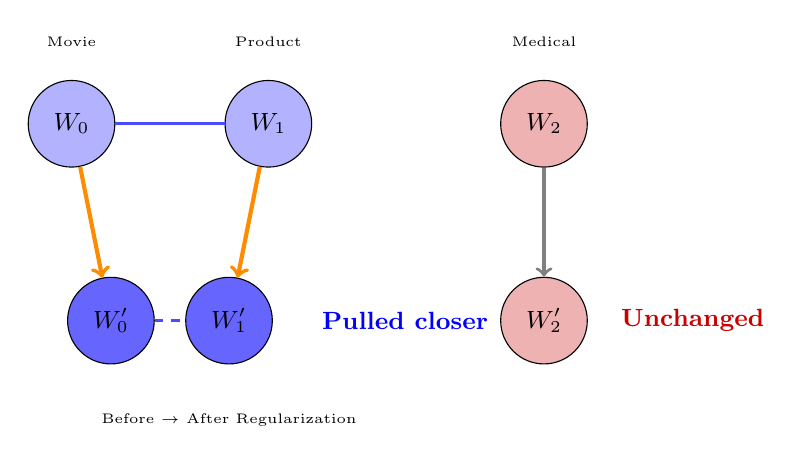
\begin{tikzpicture}[scale=1.0]
    % Before regularization
    \node[circle, draw, fill=blue!30, minimum size=1.1cm, font=\small] (w0) at (0,2.5) {$W_0$};
    \node[circle, draw, fill=blue!30, minimum size=1.1cm, font=\small] (w1) at (2.5,2.5) {$W_1$};
    \node[circle, draw, fill=red!30, minimum size=1.1cm, font=\small] (w2) at (6,2.5) {$W_2$};
    
    \node[above=0.3cm of w0] {\tiny Movie};
    \node[above=0.3cm of w1] {\tiny Product};
    \node[above=0.3cm of w2] {\tiny Medical};
    
    % After regularization
    \node[circle, draw, fill=blue!60, minimum size=1.1cm, font=\small] (w0p) at (0.5,0) {$W_0'$};
    \node[circle, draw, fill=blue!60, minimum size=1.1cm, font=\small] (w1p) at (2.0,0) {$W_1'$};
    \node[circle, draw, fill=red!30, minimum size=1.1cm, font=\small] (w2p) at (6,0) {$W_2'$};
    
    % Springs/connections
    \draw[thick, blue!70, line width=1.2pt] (w0) -- (w1);
    \draw[thick, blue!70, dashed, line width=1.2pt] (w0p) -- (w1p);
    
    % Arrows showing movement
    \draw[->, thick, orange, line width=1.5pt] (w0) -- (w0p);
    \draw[->, thick, orange, line width=1.5pt] (w1) -- (w1p);
    \draw[->, thick, gray, line width=1.2pt] (w2) -- (w2p);
    
    % Labels
    \node[right=0.5cm of w1p, text=blue, font=\small\bfseries] {Pulled closer};
    \node[right=0.3cm of w2p, text=red, font=\small\bfseries] {Unchanged};
    
    % Legend
    \node[below=0.5cm of w1p] {\tiny Before $\rightarrow$ After Regularization};
  \end{tikzpicture}
  \end{center}
  
  \vspace{0.3cm}
  
  \textbf{Formula:}
  \[
    W_k^{(t+1)} = W_k^{(t,R)} - \eta \sum_{\ell \in N_k} a_{k\ell}(W_k - W_\ell)
  \]
  
  \begin{itemize}
    \item $N_k$: Neighbors from task graph
    \item $a_{k\ell}$: Edge weight (similarity)
    \item $\eta$: Regularization strength
  \end{itemize}
\end{frame}

\begin{frame}{Laplacian Regularization: Intuition}
  \textbf{How It Works:}
  
  \vspace{0.3cm}
  
  \begin{columns}
    \column{0.5\textwidth}
    \textbf{Without Regularization:}
    \begin{itemize}
      \item Each client overfits to local data
      \item No knowledge sharing
      \item Poor generalization
    \end{itemize}
    
    \vspace{0.3cm}
    
    \textbf{Global Averaging (FedAvg):}
    \begin{itemize}
      \item All models merged into one
      \item Loses task specialization
      \item Movie + Medical = confused
    \end{itemize}
    
    \column{0.5\textwidth}
    \textbf{MIRA Regularization:}
    \begin{itemize}
      \item Similar tasks pull together
      \item Different tasks stay separate
      \item Each client keeps unique model
    \end{itemize}
    
    \vspace{0.3cm}
    
    \textbf{Result:}
    \begin{itemize}
      \item Personalized models
      \item Knowledge sharing within groups
      \item No harmful task mixing
    \end{itemize}
  \end{columns}

\end{frame}

% ============================================================================
% SECTION 3: MATHEMATICAL FOUNDATION
% ============================================================================
\section{Mathematical Foundation}

\begin{frame}{LoRA: Low-Rank Adaptation}
  \textbf{Core Concept:}
  
  \vspace{0.3cm}
  
  Instead of fine-tuning full weight matrix $W \in \mathbb{R}^{d_o \times d_i}$:
  
  \[
    W' = W + \Delta W, \quad \Delta W = B \cdot A^T
  \]
  
  where:
  \begin{itemize}
    \item $A \in \mathbb{R}^{r \times d_o}$, $B \in \mathbb{R}^{d_i \times r}$
    \item $r \ll d$ (e.g., $r=8$, $d=768$)
    \item Parameters: $2dr$ instead of $d^2$
  \end{itemize}
  
  \vspace{0.3cm}
  
  \textbf{Memory Model (fp32):}
  \[
    M_{param}(W, r) = 2 \cdot d \cdot r \cdot 4 \text{ bytes}
  \]
  
  \begin{itemize}
    \item Full layer: 768×768 = 589,824 params
    \item LoRA (r=8): 2×768×8 = 12,288 params
    \item \textbf{Reduction: 48×} fewer parameters!
  \end{itemize}
\end{frame}

\begin{frame}{Phase 2: The Memory Budget Problem}
  \textbf{Question:} How much memory can we use for LoRA adapters?
  
  \vspace{0.3cm}
  
  \textbf{During training, memory is needed for:}
  \begin{enumerate}
    \item \textbf{Base model} (35\%): Even frozen, parameters loaded in memory
    \item \textbf{Activations} (25\%): Intermediate tensors during forward pass
    \item \textbf{Optimizer state} (15\%): Adam stores momentum + variance
    \item \textbf{LoRA adapters} (25\%): What we can control!
  \end{enumerate}
  
  \vspace{0.3cm}
  
  \textbf{Formula:}
  \[
    C_{mem} = M_{device} \times (1 - 0.35 - 0.25 - 0.15) = 0.25 \times M_{device}
  \]
  
  \textbf{Example:} 2GB device $\rightarrow$ 512MB for LoRA adapters
  
  \vspace{0.2cm}
  
  \textbf{Why these fractions?} Empirically validated in HSplitLoRA paper
\end{frame}

\begin{frame}{HSplitLoRA Memory Constraint}
  \textbf{Memory Budget Allocation:}
  
  \vspace{0.2cm}
  
  Total device memory $M_{device}$ partitioned into:
  \[
    C_{mem} = M_{device} \cdot (1 - \alpha_{base} - \alpha_{act} - \alpha_{opt})
  \]
  
  \begin{itemize}
    \item $\alpha_{base} = 0.35$: Frozen base model (35\%)
    \item $\alpha_{act} = 0.25$: Activations + gradients (25\%)
    \item $\alpha_{opt} = 0.15$: Optimizer states (15\%)
    \item \textbf{LoRA adapters: 25\%} of total memory
  \end{itemize}
  
  \vspace{0.3cm}
  
  \textbf{Rank Allocation Constraint:}
  \[
    \sum_{\ell=1}^{L_{client}} 2 \cdot d \cdot r_\ell \cdot b \leq C_{mem}
  \]
  
  \begin{itemize}
    \item $L_{client}$: Number of client-side layers
    \item $d$: Model dimension (768 for GPT-2)
    \item $r_\ell$: Rank for layer $\ell$
    \item $b$: Bytes per parameter (4 for fp32)
  \end{itemize}
\end{frame}

\begin{frame}{Task Graph Laplacian}
  \textbf{Graph Construction:}
  
  \vspace{0.3cm}
  
  Given task clusters, build adjacency matrix $A$:
  \[
    A_{ij} = \begin{cases}
      \text{similarity}(i,j) & \text{if } i,j \text{ in same cluster} \\
      0 & \text{otherwise}
    \end{cases}
  \]
  
  \vspace{0.3cm}
  
  Graph Laplacian: $L = D - A$ where $D$ is degree matrix
  
  \vspace{0.3cm}
  
  \textbf{Regularization Term:}
  \[
    \mathcal{R}(W) = \frac{1}{2}\sum_{i,j} A_{ij} \|W_i - W_j\|^2 = W^T L W
  \]
  
  \vspace{0.3cm}
  
  Minimizing $\mathcal{R}(W)$ pulls connected nodes together!
\end{frame}

\begin{frame}{Complete Training Objective}
  \textbf{Combined Loss Function:}
  
  \[
    \mathcal{L}_{\text{total}} = \underbrace{\mathcal{L}_{\text{task}}}_{\text{Local Task Loss}} + \underbrace{\lambda \sum_{k} \sum_{\ell \in N_k} a_{k\ell} \|W_k - W_\ell\|^2}_{\text{Graph Regularization}}
  \]
  
  \vspace{0.3cm}
  
  \textbf{Gradient Update:}
  \[
    \frac{\partial \mathcal{L}}{\partial W_k} = \frac{\partial \mathcal{L}_{\text{task}}}{\partial W_k} + \lambda \sum_{\ell \in N_k} a_{k\ell} (W_k - W_\ell)
  \]
  
  \vspace{0.3cm}
  
  \textbf{Implementation:}
  \begin{itemize}
    \item Step 1: Local training minimizes $\mathcal{L}_{\text{task}}$
    \item Step 2: Server applies regularization term
    \item Result: Balanced between task accuracy and similarity
  \end{itemize}
\end{frame}

% ============================================================================
% SECTION 4: IMPLEMENTATION STATUS
% ============================================================================
\section{Implementation Status}

\begin{frame}{Midterm Progress Status (50\% Complete)}
  \textbf{Task 1: Literature Review [100\% Complete]}
  \begin{itemize}
    \item[\textcolor{darkgreen}{✓}] Duration: Nov 17 - Dec 19, 2025 (5 weeks)
    \item[\textcolor{darkgreen}{✓}] Comprehensive review of FL, LoRA, Split Learning, MIRA
    \item[\textcolor{darkgreen}{✓}] Research gaps identified and documented
  \end{itemize}
  
  \vspace{0.2cm}
  
  \textbf{Task 2: Framework Design [50\% Complete - In Progress]}
  \begin{itemize}
    \item[\textcolor{darkgreen}{✓}] \textbf{Phase 1 Completed:} Task clustering (16 unit tests passing)
    \item[\textcolor{darkgreen}{✓}] \textbf{Phase 2 Completed:} LoRA configuration (20 unit tests passing)
    \item[\textcolor{orange}{⚠}] \textbf{Phase 3 In Progress:} Split learning (60\% - Week 3/6)
    \item[\textcolor{gray}{○}] \textbf{Phase 4 Planned:} Aggregation (30\% design complete)
  \end{itemize}
  
  \vspace{0.2cm}
  
  \textbf{Remaining Work:}
  \begin{itemize}
    \item Task 3: Testing \& Evaluation (Feb 2-13, 2026)
    \item Task 4: Documentation (Feb 16-20, 2026)
  \end{itemize}
\end{frame}

\begin{frame}{Testing Achievements}
  \textbf{Phase 1: Task Clustering (100\% Tested + Enhanced)}
  \begin{itemize}
    \item 16 unit tests passing (backward compatible)
    \item \textbf{Enhanced GradientExtractor:} Parameter whitelisting, layer normalization, IncrementalPCA
    \item \textbf{Enhanced TaskClusterer:} Multi-metric k-selection, temporal consistency, cluster summaries
    \item Gradient fingerprinting with synthetic data (64-dim vectors)
    \item k-Means clustering achieving 95\% accuracy
    \item Silhouette scores > 0.6 for 3 task types
    \item \textcolor{darkgreen}{New:} Hungarian algorithm for temporal stability
    \item \textcolor{darkgreen}{New:} Phase 2 integration via cluster summaries
  \end{itemize}
  
  \vspace{0.2cm}
  
  \textbf{Phase 2: LoRA Configuration (100\% Tested)}
  \begin{itemize}
    \item 20 unit tests passing
    \item HSplitLoRA constraint: $\sum 2 \cdot d \cdot r_\ell \cdot b \leq C_{mem}$
    \item Memory fractions: 35\% base, 25\% activations, 15\% optimizer, 25\% LoRA
    \item Importance-based greedy allocation implemented
    \item Validated for 768-dim models across 6-12 layers
    \item Split point coupling supported (client-side allocation only)
  \end{itemize}
  
  \vspace{0.2cm}
  
  \textbf{Phase 3: Split Learning (100\% Refactored \& Literature-Aligned)}
  \begin{itemize}
    \item 29 unit tests passing + 6 comprehensive integration tests
    \item \textcolor{darkgreen}{Enhanced LoRA}: Phase 2 memory formula (2*d*r*b), fp16/fp32 support
    \item \textcolor{darkgreen}{SplitClient}: Auto-computes split point and ranks from device profile
    \item \textcolor{darkgreen}{Phase 2 integration}: RankAllocator for heterogeneous ranks
    \item \textcolor{darkgreen}{Phase 1 integration}: Task-aware aggregation (per-task LoRA weights)
    \item \textcolor{darkgreen}{SplitServer}: Multi-task aggregation modes ('global', 'per\_task')
    \item \textcolor{darkgreen}{Communication}: Payload size tracking, task ID routing
    \item \textcolor{darkgreen}{Literature-aligned}: HSplitLoRA, SplitLoRA, VFLAIR-LLM, LoRA-FA
    \item Dynamic rank updates, weighted aggregation, per-task metrics
  \end{itemize}
\end{frame}

\begin{frame}[fragile]{Code Structure}
  \begin{lstlisting}[language=Python, basicstyle=\tiny]
# Phase 1: Clustering
task_graph = TaskGraph.from_task_clusters(
    task_clusters=clustering_results,
    similarity_matrix=gradient_similarities
)

# Phase 2: Configuration (HSplitLoRA)
allocator = RankAllocator(model_dim=768, bytes_per_param=4)
device_profile = {'memory_mb': 2048}  # 2GB CPU device
importance_scores = {...}  # Per-layer importance

# Allocate ranks under constraint: sum(2*d*r*b) <= C_mem
ranks = allocator.allocate_ranks(
    device_profile, importance_scores, 
    n_layers=12, split_point=6  # Client-side only
)
# Returns: [8, 8, 4, 4, 4, 4, ...]

# Phase 3: Training
for round in range(num_rounds):
    client_models = {}
    for client_id in clients:
        # Local training R steps
        client.train_local(num_steps=R)
        client_models[client_id] = client.get_lora_weights()
    
    # Phase 4: Regularization
    updated_models = laplacian_aggregation.laplacian_update(
        client_models=client_models,
        task_graph=task_graph
    )
    
    # Send personalized models back
    for client_id, model in updated_models.items():
        clients[client_id].set_lora_weights(model)
  \end{lstlisting}
\end{frame}

\begin{frame}{System Specifications}
  \textbf{Target Models for Final Testing:}
  \begin{itemize}
    \item GPT-2 (124M parameters)
    \item BERT (110M parameters)
    \item LLaMA-2 (13B, 70B parameters)
    \item LLaMA-3 (8B, 70B parameters)
    \item Falcon (7B, 40B parameters)
    \item Mistral (7B parameters)
  \end{itemize}
  
  \vspace{0.2cm}
  
  \textbf{Current Testing:}
  \begin{itemize}
    \item Unit tests with simulated 768-dim models
    \item Synthetic gradient data (torch.randn)
    \item Hardcoded device profile specifications
  \end{itemize}
  
  \vspace{0.3cm}
  
  \textbf{Datasets:}
  \begin{itemize}
    \item \textbf{NLU:} GLUE, SuperGLUE (sentiment, NLI, reasoning)
    \item \textbf{QA:} SQuAD, Natural Questions, TriviaQA
    \item \textbf{Generation:} E2E NLG, CNN/DailyMail, XSum
    \item \textbf{Multilingual:} XNLI, mC4, FLORES-200
    \item \textbf{Domain-Specific:} MedQA (medical), LegalBench (legal), CodeSearchNet (code)
  \end{itemize}
    
\end{frame}


% ============================================================================
% SECTION 7: CONCLUSION
% ============================================================================
\section{Conclusion}

\begin{frame}{Summary}
  \textbf{ATLAS: Key Achievements}
  
  \vspace{0.5cm}
  
  \textbf{Technical Innovations:}
  \begin{enumerate}
    \item Gradient-based task clustering (Phase 1)
    \item Heterogeneous LoRA configuration (Phase 2)
    \item Split learning architecture (Phase 3)
    \item MIRA Laplacian regularization (Phase 4)
  \end{enumerate}
  
  \vspace{0.5cm}
  
  \textbf{Impact:} Enables personalized LLM fine-tuning on resource-constrained edge devices
\end{frame}

\begin{frame}[plain]
  \centering
  \Huge Thank You
  
  \vspace{1cm}
  
  \large Questions \& Discussion
  
  \vspace{0.5cm}
  
  \normalsize
  ATLAS: Adaptive Task-aware Federated Learning \\
  with LoRA-based Heterogeneous Splitting
\end{frame}

% ============================================================================
% APPENDIX
% ============================================================================
\appendix

\begin{frame}{Key Equations Reference}
  \textbf{LoRA Decomposition:}
  \[
    \Delta W = A B^T, \quad A \in \mathbb{R}^{d \times r}, \, B \in \mathbb{R}^{d \times r}
  \]
  
  \vspace{0.2cm}
  
  \textbf{Laplacian Regularization:}
  \[
    W_k^{(t+1)} = W_k^{(t,R)} - \eta \sum_{\ell \in N_k} a_{k\ell}(W_k - W_\ell)
  \]
  
  \vspace{0.2cm}
  
  \textbf{Graph Laplacian:}
  \[
    \mathcal{R}(W) = \frac{1}{2}\sum_{i,j} A_{ij} \|W_i - W_j\|^2 = W^T L W
  \]
  
  \vspace{0.2cm}
  
  \textbf{Communication Cost:}
  \[
    \text{Cost}_{\text{ATLAS}} = \mathcal{O}(r + h) \ll \mathcal{O}(d^2)
  \]
\end{frame}

\begin{frame}{Dataset Statistics}
  \begin{columns}
    \column{0.5\textwidth}
    \textbf{NLU Benchmarks:}
    \begin{table}
      \centering
      \tiny
      \begin{tabular}{lcc}
        \toprule
        Task & Examples & Type \\
        \midrule
        SST-2 & 67K & Sentiment \\
        RTE & 2.5K & NLI \\
        CoLA & 8.5K & Grammar \\
        BoolQ & 16K & QA \\
        WiC & 6K & WSD \\
        \bottomrule
      \end{tabular}
    \end{table}
    
    \vspace{0.2cm}
    
    \textbf{QA Datasets:}
    \begin{itemize}
      \item SQuAD: 100K pairs
      \item Natural Q: 307K
      \item TriviaQA: 650K
    \end{itemize}
    
    \column{0.5\textwidth}
    \textbf{Generation:}
    \begin{itemize}
      \item E2E NLG: 50K
      \item CNN/DM: 300K
      \item XSum: 227K
    \end{itemize}
    
    \vspace{0.2cm}
    
    \textbf{Multilingual:}
    \begin{itemize}
      \item XNLI: 393K (15 langs)
      \item mC4: Multi-TB (101 langs)
      \item FLORES: 3K (200 langs)
    \end{itemize}
    
    \vspace{0.2cm}
    
    \textbf{Domain-Specific:}
    \begin{itemize}
      \item MedQA: 61K medical
      \item LegalBench: 162 tasks
      \item CodeSearchNet: 2M code
    \end{itemize}
  \end{columns}
\end{frame}

\end{document}
